\documentclass[12pt]{article}
\usepackage[utf8]{inputenc}
\usepackage{float}
\usepackage{amsmath}
\usepackage{tikz}
\usepackage{cancel}
\usepackage[hmargin=3cm,vmargin=6.0cm]{geometry}
%\topmargin=0cm
\topmargin=-2cm
\addtolength{\textheight}{6.5cm}
\addtolength{\textwidth}{2.0cm}
%\setlength{\leftmargin}{-5cm}
\setlength{\oddsidemargin}{0.0cm}
\setlength{\evensidemargin}{0.0cm}

%misc libraries goes here

\begin{document}

\section*{Student Information}
%Write your full name and id number between the colon and newline
%Put one empty space character after colon and before newline
Full Name: Ahmet Eren Çolak \\
Id Number: 2587921 \\

% Write your answers below the section tags
\section*{Q. 1}

\begin{align*}
    \sum_{n=1}^{\infty} a_n \cdot x^n &= \sum_{n=1}^{\infty} (a_{n-1} + 2^n) \cdot x^n  \\
    &= \sum_{n=1}^{\infty} a_{n-1} \cdot x^n + \sum_{n=1}^{\infty} 2^n \cdot x^n \\
    &= \sum_{n=0}^{\infty} a_{n} \cdot x^{n+1} + \sum_{n=0}^{\infty} 2^{n+1} \cdot x^{n+1} \\
    &= x \sum_{n=0}^{\infty} a_n \cdot x^n + 2x\sum_{n=0}^{\infty} 2^n \cdot x^n \\
    &= x \sum_{n=0}^{\infty} a_n \cdot x^n + \frac{2x}{1-2x} \\
\end{align*}

Let $F(x)=\sum_{n=0}^{\infty} a_n \cdot x^n$:

\begin{align*}
    F(x) - a_0 &= x \cdot F(x) + \frac{2x}{1-2x}\\
    F(x)(1-x) &= \frac{2x}{1-2x} + a_0\\
    F(x) &= \frac{2x}{(1-2x)(1-x)} + \frac{a_0}{1-x}\\
    F(x) &= \frac{2x}{(1-2x)(1-x)} + a_0\sum_{n=0}^{\infty} x^n \\
\end{align*}
\\ \\ \\ \\ \\ \\ \\
Transform $\frac{2x}{(1-2x)(1-x)}$ into generating function:

\begin{align*}
    \frac{1}{1-x} = \sum_{n=0}^{\infty} x^n &\text{, } \frac{1}{1-2x} = \sum_{n=0}^{\infty} 2^nx^n \\
    \frac{1}{1-x} - \frac{1}{1-2x} &= \frac{-x}{(1-2x)(1-x)} \\
    -2\cdot(\frac{1}{1-x} - \frac{1}{1-2x}) &= \frac{2x}{1-2x} \\
    2\sum_{n=0}^{\infty} 2^n\cdot x^n - 2\sum_{n=0}^{\infty} x^n &= \frac{2x}{1-2x} \\
\end{align*}

\begin{align*}
    F(x) &= 2\sum_{n=0}^{\infty} 2^n\cdot x^n - 2\sum_{n=0}^{\infty} x^n + a_0\sum_{n=0}^{\infty} x^n \\
    F(x) &= \sum_{n=0}^{\infty} (2^{n+1} - 2 + a_0)\cdot x^n \\
    a_n &= 2^{n+1} - 2 + a_0 \\
\end{align*}

When $a_0$ is substituted $a_n = 2^{n+1} - 1$.

\section*{Q. 2}
\subsection*{a.}
\begin{center}
    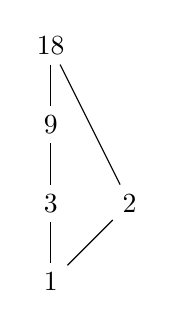
\begin{tikzpicture}
        \node (top) at (0,0) {$18$};
        \node [below of=top] (nine) {$9$};
        \node [below of=nine] (three){$3$};
        \node [right of=three] (two){$2$};
        \node [below of=three] (one){$1$};
        \draw (top) -- (nine) -- (three) -- (one);
        \draw (top) -- (two) -- (one);
    \end{tikzpicture}
\end{center}

\subsection*{b.}
\begin{equation*}
    \begin{bmatrix}
        1 & 1 & 1 & 1 & 1\\
        0 & 1 & 0 & 0 & 1\\
        0 & 0 & 1 & 1 & 1\\
        0 & 0 & 0 & 1 & 1\\
        0 & 0 & 0 & 0 & 1 
    \end{bmatrix}
\end{equation*}

\section*{Q. 3}
\subsection*{a.}
Let $A$ be a subset of natural numbers from $1$ to $n$. 
Then all possible relations are:
\begin{align*}
    &(1,1), (1,2), (1,3), \dots, (1,n) \\
    &(2,1), (2,2), (2,3), \dots, (2,n) \\
    &(3,1), (3,2), (3,3), \dots, (3,n) \\
    &\vdots \\
    &(n,1), (n,2),(n,3), \dots, (n,n) \\
\end{align*}
When relations $(a,b)$ with different entries considered together, there are $3$ options for them: $(a,b)$ or $(b,a)$ or non existent.
There are $(n^2-n) / 2$ of these relations.

When relations $(a,a)$ with same entries considered, there are $2$ options for them: existent or non existent. There are $n$ of these relations.

Therefore there are $3^{\frac{n(n-1)}{2}}\cdot2^n$ anti-symmetric relations on $A$.

\subsection*{b.}
When reflexive relations on $A$ are excluded from calculation, number of possible relations will be both reflexive and anti-symmetric.
\begin{align*}
    &\cancel{(1,1)}, (1,2), (1,3), \dots, (1,n)  \\
    &(2,1), \cancel{(2,2)}, (2,3), \dots, (2,n)  \\
    &(3,1), (3,2), \cancel{(3,3)}, \dots, (3,n) \\
    &\vdots \\
    &(n,1), (n,2), (n,3), \dots, \cancel{(n,n)} \\
\end{align*}
There are $3^{\frac{n(n-1)}{2}}$ both reflexive and anti-symmetric relations.

\end{document}
